\documentclass[a4paper,12pt]{report}
\usepackage{mathtext}
\usepackage[T2A]{fontenc}
\usepackage[utf8]{inputenc}
\usepackage[english,russian]{babel}
\usepackage{geometry}
\usepackage{listings}
\usepackage{amsmath}
\geometry{top=2cm}
\usepackage{titlesec}
\usepackage{color}
\usepackage{pgfplots}
\usepackage{filecontents}
\usetikzlibrary{datavisualization}
\usetikzlibrary{datavisualization.formats.functions}
\usepackage{caption}
\DeclareCaptionFont{white}{\color{white}}
\DeclareCaptionFormat{listing}{\colorbox{gray}{\parbox{\textwidth}{#1#2#3}}}
\captionsetup[lstlisting]{format=listing,labelfont=white,textfont=white}


% Для измененных титулов глав:
\definecolor{gray75}{gray}{0.75} % определяем цвет
\newcommand{\hsp}{\hspace{20pt}} % длина линии в 20pt
% titleformat определяет стиль
\titleformat{\chapter}[hang]{\Huge\bfseries}{\thechapter\hsp\textcolor{gray75}{|}\hsp}{0pt}{\Huge\bfseries}




\begin{document}
\begin{titlepage}
	\centering
	{\scshape\LARGE МГТУ им. Н.Э.Баумана \par}
	\vspace{4cm}
	{\scshape\LargeРубежный контроль\par}
	\vspace{0.5cm}	
	{\scshape\Large По курсу: "Анализ алгоритмов"\par}
	\vspace{2cm}
	{\huge\bfseriesМетоды анализа тональности текстов\par}
	\vspace{3cm}
	\Large Работу выполнил: Луговой Дмитрий, ИУ7-51Б\par
	\vspace{0.5cm}
	\Large Преподаватель:  Волкова Л.Л.\par

	\vfill
	\large \textit {Москва, 2019} \par
\end{titlepage}

\setcounter{page}{2}

\tableofcontents

\newpage
\chapter*{Введение}
\addcontentsline{toc}{chapter}{Введение}
\hspace{0.6cm} \textbf{Цель работы}: изучение методов анализа эмоциональной окраски(тональности) текстов.\\\\

\textbf{\LARGE Задачи работы}\\\\
\begin{enumerate}
\item[1)] Изучить существующие методы анализа тональности текстов;
\item[2)] Провести сравнительный анализ найденных методов.
\end{enumerate}

\chapter{Аналитическая часть}
\hspace{0.6cm}В данном разделе содержатся описания методов анализа тональности текста и производится их сравнительный анализ.

\section{Тональность текста}
\hspace{0.6cm}\textbf{Тональность} — это эмоциональное отношение автора высказывания к некоторому объекту (объекту реального мира, событию, процессу или их свойствам/атрибутам), выраженное в тексте. Эмоциональная составляющая, выраженная на уровне лексемы или коммуникативного фрагмента, называется лексической тональностью (или лексическим сентиментом). Тональность всего текста в целом можно определить как функцию (в простейшем случае сумму) лексических тональностей составляющих его единиц (предложений) и правил их сочетания.

Анализ тональности текста (сентимент-анализ) — класс методов контент-анализа в компьютерной лингвистике, предназначенный для автоматизированного выявления в текстах эмоционально окрашенной лексики и эмоциональной оценки авторов (мнений) по отношению к объектам, речь о которых идёт в текст.

Основной целью анализа тональности является нахождение мнений в тексте и выявление их свойств. Какие именно свойства будут исследоваться, зависит уже от поставленной задачи.\\
Виды тональных оценок:
\begin{itemize}
\item позитивная;
\item негативная;
\item нейтральная.
\end{itemize}
\hspace{0.6cm}Под «нейтральной» подразумевается, что текст не содержит эмоциональной окраски. \\
Классификация текстов применяется, в том числе, для:
\begin{itemize}
\item Разделения веб страниц и сайтов по тематическим каталогам;
\item Борьбы со спамом;
\item Определение языка текста;
\item Показа более релевантной рекламы;
\end{itemize}
\section{Классификация методов анализа}
\hspace{0.6cm}Методы анализа классифицируются на:
\begin{itemize}

\item \textbf{Методы, основанные на правилах и словарях}

\hspace{0.6cm}Эти методы основаны на поиске тональности в тексте по заранее составленным тональным словарям и правилам с применением лингвистического анализа. По совокупности найденной эмотивной лексики текст может быть оценен по шкале, содержащей количество негативной и позитивной лексики. Данный метод может использовать как списки правил, подставляемые в регулярные выражения, так и специальные правила соединения тональной лексики внутри предложения.

\hspace{0.6cm}Однако процесс создания этих «фолиантов» очень трудоемкий; основной проблемой является тот факт, что одно и то же слово в разных контекстах может обладать различной тональностью. Это означает, что для адекватной работы системы требуется составить большое количество правил – поэтому чаще всего системы анализа тональности текста создаются с привязкой к определенной предметной области.\\

\item \textbf{Методы, основанные на теоретико-графовых моделях}

\hspace{0.6cm}В основе этих методов используется предположение о том, что не все слова в текстовом корпусе документа равнозначны. Какие-то слова имеют больший вес и сильнее влияют на тональность текста.\\ 
При использовании этих методов анализ тональности разбивается на несколько этапов:
\begin{enumerate}
\item построение графа на основе исследуемого текста;
\item ранжирование его вершин;
\item классификация найденных слов;
\item вычисление результата.
\end{enumerate}
\hspace{0.6cm}После ранжирования вершин графа слова классифицируются в соответствии со словарем тональности, где каждому слову присваивается определенная характеристика («положительное», «отрицательное» или «нейтральное»). Результат вычисляется как соотношение количества слов с положительной оценкой к количеству слов с отрицательной оценкой.\\
\item \textbf{Методы, основанные на машинном обучении}

\hspace{0.6cm}В наше время наиболее часто используемыми в исследованиях методами являются методы на основе машинного обучения с учителем. Сутью таких методов является то, что на первом этапе обучается машинный классификатор на заранее размеченных текстах, а затем используют полученную модель при анализе новых документов.\\
Наиболее популярным является метод с "наивным байессовским" классификатором. Краткий алгоритм:
\begin{enumerate}
\item Собирается коллекция документов, на основе которой обучается машинный классификатор;
\item Каждый документ раскладывается в виде вектора признаков(аспектов), по которым он будет исследоваться;
\item Указывается правильный тип тональности для каждого документа;
\item Производится выбор алгоритма классификации и метод для обучения классификатора;
\item Полученная модель используется для определения тональности документов новой коллекции.
\end{enumerate}
\hspace{0.6cm}Также распространены методы без учителя, в основе которых лежит идея, что термины, которые чаще встречаются в этом тексте и в то же время присутствуют в небольшом количестве текстов во всей коллекции, имеют наибольший вес в тексте. Выделив данные термины, а затем определив их тональность, можно сделать вывод о тональности всего текста. Для выделения может быть использована модель TFIDF.
Иногда слова могут встречаться во многих документах текстовой коллекции. Следовательно, они не могут характеризовать принадлежность документа тому или иному классу, так как не являются ключевыми. Поэтому вводится так называемая мера IDF (обратная частота документа), которая понижает значимость частотных слов.
\begin{align}
IDF = \ln(\frac{D}{d}),
\end{align}
где D — количество всех документов, d — количество документов, в которых содержится данное слово. Таким образом, чем чаще слово встречается, тем меньше его IDF.
Мера TF (term frequency) — отношение частоты некоторого слова к общему числу слов в документе. Мера оценивает важность слов в пределах документа.
TFIDF равен произведению TF и IDF. Таким образом, TF является повышающим множителем, а IDF — понижающим. Больший вес получат слова, которые часто встречаются в одном документе, но редко в других.
\end{itemize}

\section{Анализ методов}
\hspace{0.6cm}Точность и качество системы анализа тональности текста оценивается тем, насколько хорошо она согласуется с мнением человека относительно эмоциональной оценки исследуемого текста. Для этого могут использоваться такие метрики как точность и полнота. \\
Формула для нахождения полноты:
\begin{align}
R = \frac {\text{correctly extracted opinions}}{\text{total number of opinions}}
\end{align}
где correctly extracted opinions — верно определённые мнения, total number of opinions — общее количество мнений(как найденных системой, так и не найденных).\\
 Точность вычисляется по формуле:
\begin{align}
P=\frac {\text{correctly extracted opinions}}{\text{total number of opinions found by system}}
\end{align}
где correctly extracted opinions — верно определённые мнения, total number of opinions found by system — общее количество мнений найденных системой.\\
\hspace{0.6cm}Таким образом, точность выражает количество исследуемых текстов, предложений или документов, в оценке которых мнение системы анализа тональности совпало с мнением эксперта. При этом, согласно исследованию, эксперты обычно соглашаются в оценках тональности конкретного текста в 79 \% случаев. Следовательно, программа, которая определяет тональность текста с точностью 70 \%, делает это почти так же хорошо, как и человек.

Задача определения полярности сообщений, текстов или предложений имеет множество эффективных методов решения, в каждом из которых есть особенности.

Словарные методы не позволяют создать универсальный словарь терминов, так как их вес в разных предметных областях может значительно отличаться или быть противоположным.

Методы обучения с учителем сложны составлением тренировочного словаря для предметной области, в которой используется классификатор, но в тоже время показывают наиболее высокую точность анализа.

На рис. 1.1 представлена сравнительная характеристика наиболее распространенных
методов анализа тональности.
\begin{figure}[ht!]
\center{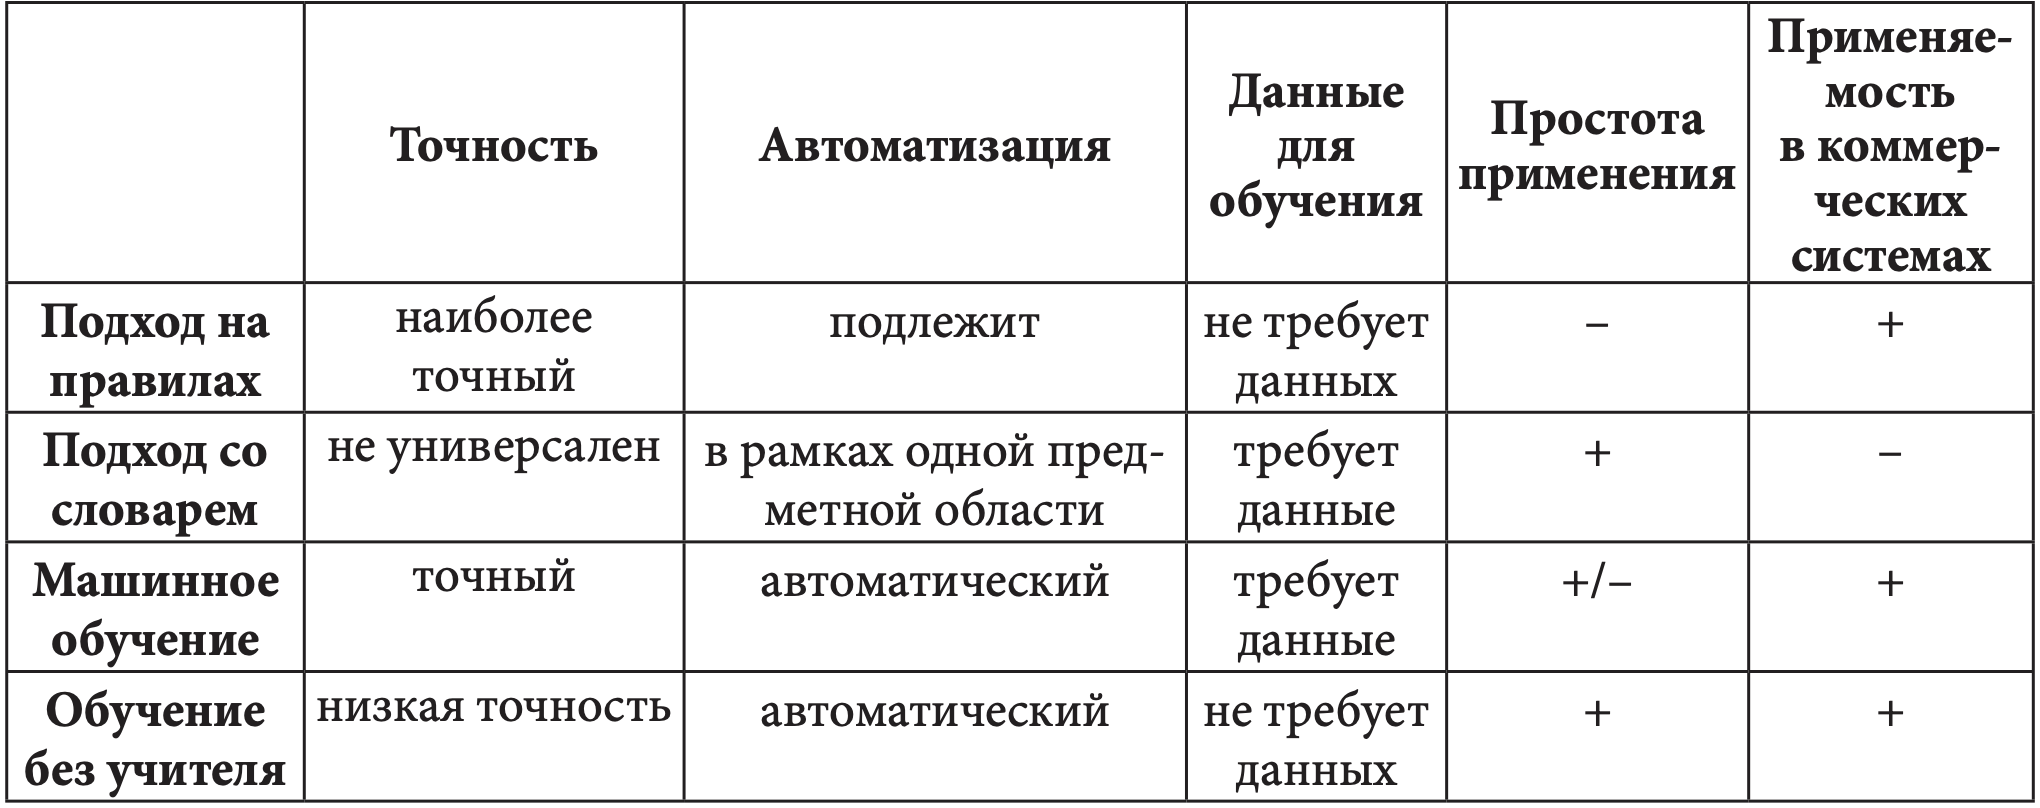
\includegraphics[scale=0.42]{Compare.png}}
\caption{Сравнение методов анализа тональности текста}
\end{figure}
\newpage
\chapter*{Заключение}
\addcontentsline{toc}{chapter}{Заключение}
\hspace{0.6cm}На основании проведенного анализа оптимальным является метод машинного обучения с учителем
с использованием наивного байесовского классификатора. Выбор метода обусловлен тем, что данный метод позволяет работать с различными исходными массивами данных для обучения системы, что может значительно повлиять на точность анализа. Также этот метод не зависит от специфики текста и может использоваться в очень широком спектре задач.
\hspace{0.6cm} 

\addcontentsline{toc}{chapter}{Список литературы}
\renewcommand\bibname{Список литературы}
\begin{thebibliography}{2} 
\bibitem{itmo} ИТМО Классификация текстов и анализ тонатльности [Электронный ресурс]. – Режим доступа: URL: http://neerc.ifmo.ru/wiki/index.php?title= \\Классификация\_текстов\_и\_анализ\_тональности. – (Дата обращения: 21.11.2019)
\bibitem{wiki} Wikipedia Анализ тональности текста [Электронный ресурс]. – Режим доступа: URL: https://ru.wikipedia.org/wiki/Анализ\_тональности\_текста. – (Дата обращения: 21.11.2019)
\bibitem{voronej} Анализ эмоциональной окраски сообщений
в социальных сетях (на примере сети «Вконтакте») [Текст]  / И. Е. Воронина, В. А. Гончаров // ВЕСТНИК ВГУ, СЕРИЯ: СИСТЕМНЫЙ АНАЛИЗ И ИНФОРМАЦИОННЫЕ ТЕХНОЛОГИИ. – 2015. - № 4. – С. 151-158.
\end{thebibliography}

\end{document}